\section{Peak and Minimum Counts} 
\label{sec:peak_min_counts}
Peaks and minima in the convergence field correspond to localized over-densities and under-densities, respectively. Counting these extrema provides valuable information about the non-Gaussian features of the matter distribution and can be used to constrain cosmological models.We adopt the formalism presented in \citet{1986ApJ...304...15B}, \citet{2016MNRAS.463.3653K} and \citet{2018MNRAS.474..712M} to rigorously describe the peak and minimum counts in the convergence field.

\subsection{Identification of Peaks and Minima}
To effectively identify peaks and minima while suppressing noise and small-scale fluctuations, the convergence map $\kappa(\hat{\mathbf{n}})$ is first smoothed with a Gaussian kernel. The smoothed convergence field, $\kappa_{\mathrm{smooth}}(\hat{\mathbf{n}})$, is defined as:
\begin{equation}
    \kappa_{\mathrm{smooth}}(\hat{\mathbf{n}}) = \int_{S^2} \kappa(\hat{\mathbf{n}}') W(\hat{\mathbf{n}} - \hat{\mathbf{n}}') \, d\hat{\mathbf{n}}',
    \label{eq:smoothing}
\end{equation}
where $W(\theta)$ is the Gaussian smoothing kernel given by:
\begin{equation}
    W(\theta) = \frac{1}{2\pi \sigma_{\theta}^2} \exp\left( -\frac{\theta^2}{2 \sigma_{\theta}^2} \right),
    \label{eq:gaussian_kernel}
\end{equation}
with $\theta = \arccos(\hat{\mathbf{n}} \cdot \hat{\mathbf{n}}')$ representing the angular separation between the points $\hat{\mathbf{n}}$ and $\hat{\mathbf{n}}'$ on the unit sphere $S^2$, and $\sigma_{\theta}$ is the smoothing scale.

To standardize the statistical analysis, the smoothed convergence values are normalized by their standard deviation. The normalized smoothed convergence, $\tilde{\kappa}_{\mathrm{smooth}, i}$, is defined as:
\begin{equation}
    \tilde{\kappa}_{\mathrm{smooth}, i} = \frac{\kappa_{\mathrm{smooth}, i} - \langle \kappa_{\mathrm{smooth}} \rangle}{\sigma_{\mathrm{smooth}}},
    \label{eq:kappa_smooth_normalized}
\end{equation}
where:
\begin{equation}
    \langle \kappa_{\mathrm{smooth}} \rangle = \frac{1}{N_{\mathrm{pix}}} \sum_{i=1}^{N_{\mathrm{pix}}} \kappa_{\mathrm{smooth}, i}, \quad \sigma_{\mathrm{smooth}}^2 = \sigma_{\mathrm{signal}}^2 + \sigma_{\mathrm{noise}}^2.
    \label{eq:normalization}
\end{equation}

A pixel $i$ in the smoothed convergence map is identified as a peak or a minimum based on the comparison of its value with its neighboring pixels. Formally, let $\mathcal{N}(i)$ denote the set of neighboring pixels of pixel $i$. Then:
\begin{align}
    \text{Peak Condition:} \quad & \kappa_{\mathrm{smooth}, i} > \kappa_{\mathrm{smooth}, j} \quad \forall \, j \in \mathcal{N}(i), \label{eq:peak_condition} \\
    \text{Minimum Condition:} \quad & \kappa_{\mathrm{smooth}, i} < \kappa_{\mathrm{smooth}, j} \quad \forall \, j \in \mathcal{N}(i). \label{eq:min_condition}
\end{align}
These conditions ensure that peaks are local maxima and minima are local minima in the convergence field.
Figure~\ref{fig:peak_min} illustrates the identification of peaks (red circles) and minima (blue circles) in the smoothed convergence map $\kappa_{\mathrm{smooth}}(\hat{\mathbf{n}})$.
\begin{figure}[ht]
    \centering
    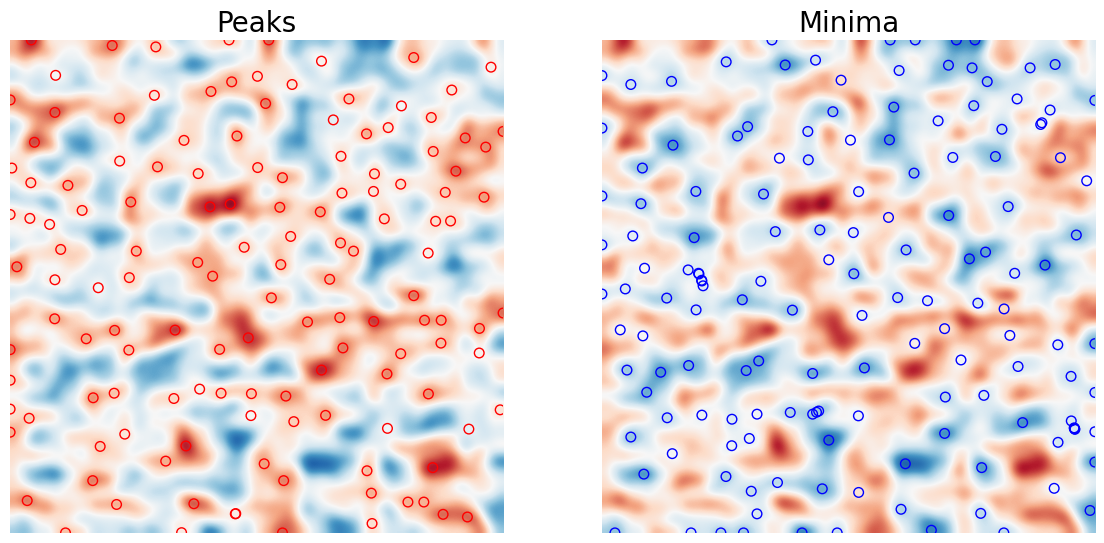
\includegraphics[width=0.8\textwidth]{figures/peaks_minima.png}
    \caption{Identification of peaks and minima in a smoothed convergence map. The left panel shows the smoothed convergence field $\kappa_{\mathrm{smooth}}(\hat{\mathbf{n}})$ with peaks (red circles) satisfying the peak condition (Equation~\eqref{eq:peak_condition}), and the right panel highlights the minima (blue circles) satisfying the minimum condition (Equation~\eqref{eq:min_condition}).}
    \label{fig:peak_min}
\end{figure}

\subsection{Peaks of Gaussian Random Fields}
For a Gaussian random field (GRF), the statistics of peaks and minima can be analytically derived. The expected number density of peaks above a threshold $\nu$ in a GRF is given by:
\begin{equation}
    N_{\mathrm{peak}}(\nu) = \frac{1}{(2\pi)^{3/2} R_*^3} e^{-\nu^2/2} \left[ \nu^2 - 1 \right],
    \label{eq:bbks_peak}
\end{equation}
where $\nu = \tilde{\kappa}_{\mathrm{smooth}}$, and $R_*$ is a characteristic scale defined by:
\begin{equation}
    R_*^2 = \frac{\langle |\nabla \kappa_{\mathrm{smooth}}|^2 \rangle}{\langle \kappa_{\mathrm{smooth}}^2 \rangle}.
    \label{eq:R_star}
\end{equation}
Similarly, the expected number density of minima below $-\nu$ is:
\begin{equation}
    N_{\mathrm{min}}(-\nu) = N_{\mathrm{peak}}(\nu).
    \label{eq:bbks_min}
\end{equation}

\begin{comment}
In particular, the local maxima
and minima on convergence maps are associated with massive haloes
and emptiest regions (voids) in our universe. The study of such
peaks and minima is highly sensitive to non-linear structures and a
complementary probe to constrain S8 (Liu et al. 2015a, b; Kacprzak
et al. 2016; Martinet et al. 2018; Shan et al. 2018; Coulton et al.
2020; Davies et al. 2021; Harnois-Deraps ´ et al. 2021; Davies et al.
2022; Zurcher ¨ et al. 2022; Liu et al. 2023).

measurements of peaks and
minima (Davies et al. 2022; Zürcher et al. 2022; Liu et al. 2023a;
Marques et al. 2024),
\end{comment}

